\chapter{Interpretation der Ergebnisse (VR)}

\section{Höhenruder Trimmkurve}

Aus den aufgezeichneten Daten lässt sich ein linearer Zusammenhang zwischen dem Anstellwinkel alpha und dem 
Höhenruderausschlag $\eta$ feststellen. Mit steigendem Höhenruderausschlag sinkt der Anstellwinkel. 
Der Anstellwinkel $\alpha$ beschreibt den Winkel zwischen dem Fluggeschwindigkeitsvektor und der Flugzeuglängsachse. Ein positiver Winkel $\alpha$ bedeutet, dass die Flugzeuglängsachse positiv gegenüber dem Fluggeschwindigkeitsvektor gedreht ist. 

\begin{figure}[h]
		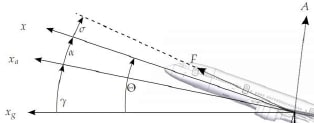
\includegraphics{./Bilder/Anstellwinkel_Definition.jpg}
	\caption{Definition Anstellwinkel}
	\label{alpha_def}
\end{figure}

Der Winkel des Höhenruders $\eta$ beschreibt die Auslenkung des Ruders gegenüber einer Neutrallage. Ein negativer 
Höhenruderausschlag bedeutet eine lokale Absenkung des Auftriebs am Höhenleitwerk, sodass es zum Absinken des Hecks kommt (Nose-up). In die positive Richtung ausgeschlagen steigt der Auftrieb am Höhenleitwerk, sodass sich das Heck hebt (Nosedown). 
Damit decken sich die Messdaten der Do 28 zu Anstellwinkel und Höhenruderausschlag mit der Theorie.




\section{Auftriebsbeiwert über Anstellwinkel}

Der Auftriebsbeiwert $C_A$ steigt linear mit zunehmendem Anstellwinkel alpha. Bei einem Anstellwinkel von $0 \ ^{\circ}$ beträgt der Auftriebsbeiwert $C_{A0}=0,2234$. Der Nullauftriebswinkel $\alpha_{0}$ ist mit $2,894 \ ^{\circ}$ der Winkel, an dem kein Auftrieb mehr erzeugt wird. Der Auftriebsanstieg $C_{A\alpha}$ berechnet sich wie folgt:

\begin{equation}
C_{A\alpha}=\frac{dC_A}{\alpha}=0,0772
\end{equation}

	
Bei der Anströmung eines Tragflügels wird die Luft umgelenkt und es entsteht eine Druckdifferenz zwischen Tragflügelober- und Oberseite, was als Voraussetzung für die Entstehung von Auftrieb ist. Der Anstellwinkel des Flügels ist dabei der größte Einflussfaktor für den Auftriebsbeiwert. Für kleine Winkel $\alpha$ mit anliegender Strömung gilt daher der lineare Zusammenhang

\begin{equation}
C_A=C_{A\alpha} \left(\alpha - \alpha_0\right)
\end{equation}

Damit stimmen die Messdaten mit der Theorie überein. Jedoch lassen sich keine Aussagen über den maximalen Auftriebsbeiwert treffen, da die aufgenommenen Anstellwinkel im Bereich der anliegenden Strömung liegen und der höchste Auftriebsbeiwert erst kurz vor dem Abreißen der Strömung erreicht wird. 

\section{Lilienthal-Polare}

\textbf{Do 128}

Die für $C_A$ und $C_W$ errechneten Werte werden für die Erstellung der Lilienthalpolare gegeneinander aufgetragen und mit einer quadratischen Regression angenähert. Daraus ergibt sich für den Nullwiderstand $C_{W0}$ ein Wert von 0,0503, für den Polynomterm erster Ordnung ein Koeffizient von 0,0033 und für den zweiten Grades ein Koeffizient von 0,0258. 
Aus der Lillienthal-Polare lässt sich die minimale reziproke Gleitzahl ermitteln, die die Höhendifferenz beim Sinken des Flugzeugs bei einer bestimmten Flugstrecke beschreibt. Zur Ermittlung der minimalen reziproken Gleitzahl wird eine Tangente durch den Ursprung an die entstandene Polare gelegt. Am Schnittpunkt der Tangente mit der Polaren können die zugehörigen Beiwerte $C_A^*=$1,39 und  $C_W^*$=0,105 abgelesen werden, mit denen die reziproke Steigung der Tangente mit

\begin{equation}
\epsilon_{min} =  \frac {C_{W}^{\ast}} {C_{A}^{\ast}} = \frac{0,105} {1,39}=0,0755
\end{equation}

berechnet werden kann. Der Gleitwinkel $\gamma$, der die Drehung des Geschwindigkeitsvektor gegenüber der geodätischen Horizontalebene in x-Richtung beschreibt, ergibt sich zu

\begin{equation}
\gamma=\arctan \left(-\frac{C^{*}_W}{C^{*}_A} \right)= \arctan \left(-\frac{0,105}{1,39} \right)= -4,32 \ ^{\circ}  
\end{equation}

Aus den bekannten Werten $C_{W0}$ und $C^{*}_A$ lässt sich der Widerstandsanstieg k wie folgt berechnen: 

%\[k= \(C_W0\) \div  \(C^{*} _A\)^{2}=0,0451 \div 1,39^{2}=0,2334 \] \\

 In der Theorie wird an dieser Stelle ein positiver Wert für k erwartet, was bedeutet, dass die aus der Regression entnommenen Werte falsch sind. Da nur vier verschiedene Flugzustände aufgenommen werden konnten, ist die Regression außerhalb des Messwertbereichs ungenau. \\

\textbf{Do 28}

Bei der Regression der Messpunkte der Do 28 mit einer quadratischen Polare ergibt sich für den Nullwiderstand $C_{W0}$ ein Wert von 0,0678, für den den Koeffizient des Polynomterms erster Ordnung ein Wert von -0,0441 und für den Koeffizienten zweiter Ordnung ein Wert von 0,0642. Die minimale reziproke Gleitzahl berechnet sich somit wie bei der Do 128 mit den Werten 
$C^{*}_A=1,045$ und $C^{*}_W=0,09619$ zu $\epsilon_{min}=0,09$. 
Der dazugehörige Gleitwinkel $\gamma$ berechnet sich zu $-5 \ ^{\circ}$. 

\section{Widerstand über Fluggeschwindigkeit}

\textbf{Do 128}

Der aus den Messdaten errechnete Widerstand wird über die aus den Flugversuchen ermittelte Geschwindigkeit aufgetragen. Es lässt sich beobachten, dass der Widerstand exponentiell mit steigender Geschwindigkeit wächst. \\
Der Gesamtwiderstand eines Flugzeugs setzt sich zusammen aus dem Null- und Auftriebswiderstand. Während der Nullwiderstand mit steigender Geschwindigkeit exponentiell zunimmt, nimmt der Auftriebswiderstand exponentiell ab. Die Addition beider Kurven bildet den Gesamtwiderstand, der parabelähnlich nach oben geöffnet ist und einen Tiefpunkt besitzt. An diesem Minimum bewegt sich das Flugzeug mit der optimalen Geschwindigkeit $V_{opt}$. Eine niedrigere oder höhere Geschwindigkeit würde einen Anstieg des Gesamtwiderstands bedeuten. Hier wurde $V_{opt}$ rechnerisch mit der Gleichung \ref{eq:V_opt} berechnet und hat den Wert 42,94. Im Graphen wäre das Minimum nicht ablesbar, da im Flugversuch nicht langsamer als $42 \ \frac{m}{s}$ geflogen wurde. Somit lassen sich auch keine Aussagen zum Widerstand im langsameren Flugbereichen treffen. Der minimale Widerstand $W_{min}$ kann mit \ref{eq:W_min} zu 2636,3 N berechnet werden. Damit liegt der minimale Widerstand deutlich unter den errechneten Werten für den Widerstand und könnte nicht durch graphische Auswertung ermittelt werden.

\textbf{Do 28}

Im Vergleich zu den Messwerten der Do 128 streuen die Werte viel mehr, sodass der aus der Theorie zu erwartende Verlauf schwieriger zu erkennen ist. Für die optimale Geschwindigkeit $V_{opt}$ errechnet sich aus obiger Formel ein Wert von $44,92 \ \frac{m}{s}$ und für den minimalen Widerstand $W_{min}=4678,4 \ N$. Damit liegt der minimale Widerstand deutlich über dem aus den Messchrieben errechnete Minimalwert. Dies lässt darauf zurückführen, dass der aus der Lilienthal-Polare entnommene Nullwiderstandsbeiwert $C_{W0}$ vergleichsweise hoch ausfällt. 


\section{Staudruck über Anstellwinkel}
tbd

\section{Fluggeschwindigkeit über Anstellwinkel}
tbd
